\documentclass{article}
\usepackage[utf8]{inputenc}
\usepackage{amsmath}
\usepackage{amssymb}
\usepackage{color}
\usepackage{enumitem}
\usepackage{fancyhdr}
\usepackage[margin=1in,top=1in,headheight=18pt]{geometry}
\usepackage{listings}
\usepackage{graphicx}
\usepackage{hyperref}
\usepackage{dirtree}
\usepackage{tikzsymbols}
\usepackage{wrapfig}
\usepackage{tikz}
\usepackage{soul}
\usepackage[toc,page]{appendix}
\usepackage[style=authoryear-icomp,maxbibnames=9,maxcitenames=2,backend=biber]{biblatex}
\addbibresource{./Authors.bib}
% \bibliographystyle{plainnat}
\graphicspath{ {./images/} }

\newcommand{\ExternalLink}{%
    \tikz[x=1.2ex, y=1.2ex, baseline=-0.05ex]{% 
        \begin{scope}[x=1ex, y=1ex]
            \clip (-0.1,-0.1) 
                --++ (-0, 1.2) 
                --++ (0.6, 0) 
                --++ (0, -0.6) 
                --++ (0.6, 0) 
                --++ (0, -1);
            \path[draw, 
                line width = 0.5, 
                rounded corners=0.5] 
                (0,0) rectangle (1,1);
        \end{scope}
        \path[draw, line width = 0.5] (0.5, 0.5) 
            -- (1, 1);
        \path[draw, line width = 0.5] (0.6, 1) 
            -- (1, 1) -- (1, 0.6);
        }
    }


\definecolor{ao}{rgb}{0.0, 0.0, 1.0}
\hypersetup{
    colorlinks=false,
}

\urlstyle{same}

\setlength{\parindent}{0pt}

\newcommand{\ttt}[1]{\texttt{#1}}

\title{Assignment 1 Part 2 - Phoneme Recognition}
\author{Introduction to Deep Learning \\ Emeritus \& Carnegie Mellon University}
\date{} \\
\vspace{.1in}

\begin{document}
\pagenumbering{arabic}

\maketitle

\section{Overview}
In this assignment, we'll be tackling a real-world application of DL using the official PyTorch.\\

\textbf{Objective}: Our task is from the domain of speech recognition. Given audio of human speech, our network will attempt to classify the ``phoneme" being spoken at each 25ms frame of audio. \\

\noindent\fbox{%
    \parbox{\textwidth}{%
        \textbf{Note}: We recommend you start this assignment early. While understanding the concepts and writing the code may not take more than a few hours, total training time may take $>$ 4 (although you can be AFK for much of it). \\
        
        That said, to save you some time, we provide advice and guidelines on selecting architectures/hyperparams. You hopefully won't need to train more than 2 models. \\
        
        In practice, people can end up training dozens to thousands of models in order to find good architectures and hyperparams. Even with dozens of GPUs, this can take weeks. But almost all of those models lead to dead-ends. Our suggestions will still give you a good taste of what choices matter without wasting your time
    }%
}

\vspace{5mm}

Before we dive in, let's cover a few important concepts. \\

\textbf{Note}: You may have noticed that deep learning involves a \textit{lot} of reading and misc domain knowledge. This never changes, even after you get more comfortable with DL. If anything, you read MORE the deeper you go. So you'll have to get used to powering through readings; you can do it!

\newpage
% --------------------------------------

\subsection{Background: Prepping audio data for phoneme classification}

We'll first cover how audio data is typically prepped for speech processing tasks. \\

Raw audio data (i.e. a `speech waveform') is a sequence of numbers that represent the amplitude of the sound wave at each time step. \\

\begin{figure}[h]
\centering
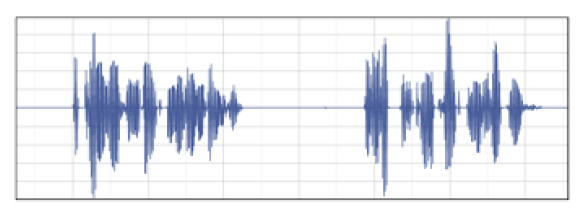
\includegraphics[width=0.4\textwidth]{images/raw_audio.png}
\caption{Typical example of raw audio data. X axis is time step and Y axis is amplitude.}
\end{figure}

However, for various reasons, this raw 1D signal generally isn't great for speech processing applications. So we convert this data to a \textbf{mel-frequency spectrogram}.

\newpage

\subsubsection{Spectrograms}
A \textbf{spectrogram} represents a signal across time decomposed into amplitudes of individual frequencies. \\

One reason we prefer spectrograms over raw audio is that raw audio only tells us the total amplitude at each time. But the amplitude of each individual frequency may be super informative. So we convert to spectrograms to have that info readily available. \\

\begin{figure}[h]
    \centering
    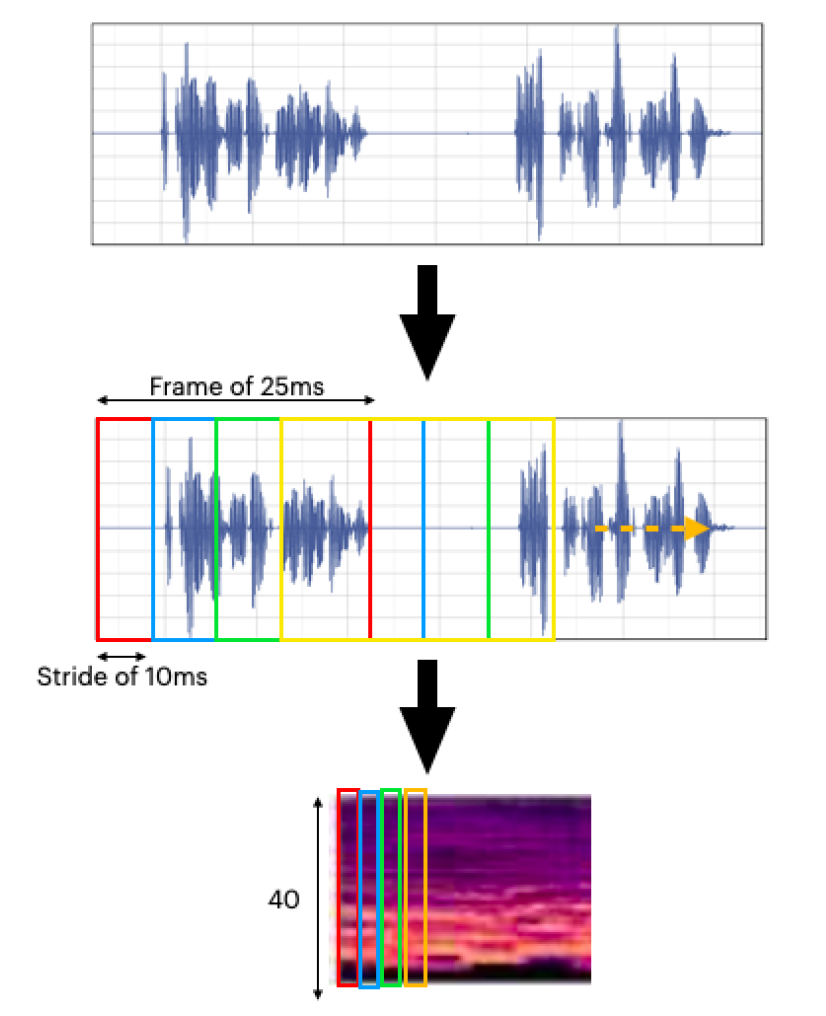
\includegraphics[width=0.5\textwidth]{images/spectrogram_conversion.png}
    \caption{Converting raw audio to a spectrogram.}
\end{figure}

Without getting into too much depth, this is the general process for how this conversion happens:

\begin{enumerate}
    \item We split the raw data into overlapping ``frames" of pre-defined duration.
        \begin{itemize}
            \item We define each frame size (here 25ms) and the `stride' (here 10ms).
            \item Starting from the beginning of the signal, we grab a frame covering 25ms, then move forward 10ms after the beginning of this frame and grab another frame covering 25ms.
            \item Notice each frame slightly overlaps with its neighbors.
        \end{itemize}
    \item We perform a \underline{\href{https://en.wikipedia.org/wiki/Fourier_transform}{Fourier transform \ExternalLink}} on each frame.
    \item We apply filters to extract the amplitude of each frequency band (typically 40 total filters for 40 total frequency bands).
\end{enumerate}

So a 10 second audio clip would get converted into a matrix shaped \ttt{(1000, 40)}. We get 1000 because a stride of 10ms means we'll get 100 frames per second, and there are 10 seconds. \ttt{100 * 10 = 1000}. We get 40 because of the 40 frequency bands extracted. \\

If you're interested in the details of the process, you can read about it \underline{\href{https://haythamfayek.com/2016/04/21/speech-processing-for-machine-learning.html}{here \ExternalLink}}. \\

\newpage
% --------------------------------------
\subsubsection{Mel-Frequency}

To improve suitability for speech even further, we can adjust how we define each filter according to the \textbf{Mel-scale}. This scale adjusts the relative strength of each frequency band to mimic the logarithmic way that humans perceive sound. Like your own hearing, this scale will emphasize lower frequencies and de-emphasize higher ones. \\

Now we have mel-frequency spectrograms! \\

\textbf{Note}: We've already converted the data to mel-spectrograms for you. But we still cover all this to make sure you understand, end-to-end, how this pipeline works.

\subsection{Background: Phonemes}
Now let's introduce \textbf{phonemes}, which are the labels of our problem. \\

Phonemes are indivisible units of human speech. Just like how English writing can be viewed as a sequence of letters, speech can be viewed as a sequence of phonemes. \\

For our problem, we'll be classifying each frame as being one of 71 possible sounds and phonemes:

\begin{verbatim}
   [`SIL', `SPN', `AA0', `AA1', `AA2', `AE0', `AE1', `AE2', `AH0',
   `AH1', `AH2', `AO0', `AO1', `AO2', `AW0', `AW1', `AW2', `AY0', `AY1',
   `AY2', `B', `CH', `D', `DH', `EH0', `EH1', `EH2', `ER0', `ER1', 
   `ER2', `EY0', `EY1', `EY2', `F', `G', `HH', `IH0', `IH1', `IH2',
   `IY0', `IY1', `IY2', `JH', `K', `L', `M', `N', `NG', `OW0', `OW1',
   `OW2', `OY0', `OY1', `OY2', `P', `R', `S', `SH', `T', `TH', `UH0',
   `UH1', `UH2', `UW0', `UW1', `UW2', `V', `W', `Y', `Z', `ZH']
\end{verbatim}

Some notes:
\begin{itemize}
    \item \ttt{`SIL'} represents silence (no phonemes being spoken)
    \item \ttt{`SPN'} represents an unknown sound (like a cough)
    \item Phonemes with a number after them (i.e. `\ttt{OW2}') indicate similar but slightly different variations of a phoneme.
    \item There isn't necessarily one gold-standard set of phonemes for a single language. Different datasets and languages you see in the future may use different phonemes.
\end{itemize}

Here are some examples of spoken words broken down into phonemes:

\begin{verbatim}
    Erupt: IH0 R AH1 P T
    Existant: EH0 G Z IH1 S T AH0 N T
    Twitter: T W IH1 T AH R
\end{verbatim}

If you want any additional info, these two Wikipedia articles are excellent:

\begin{enumerate}
    \item \underline{\href{https://en.wikipedia.org/wiki/Phoneme}{Phoneme \ExternalLink}}
    \item \underline{\href{https://en.wikipedia.org/wiki/English_phonology}{English Phonology \ExternalLink}}
\end{enumerate}

% --------------------------------------
\newpage

\section{Classifying Phonemes}
Almost there! \\

Now that we understand our data (mel-spectrograms) and labels (phonemes), we can more precisely state our goal. \\

\textbf{Objective}: Identify the phoneme being spoken for every frame in the dataset. \\

\begin{figure}[h]
    \centering
    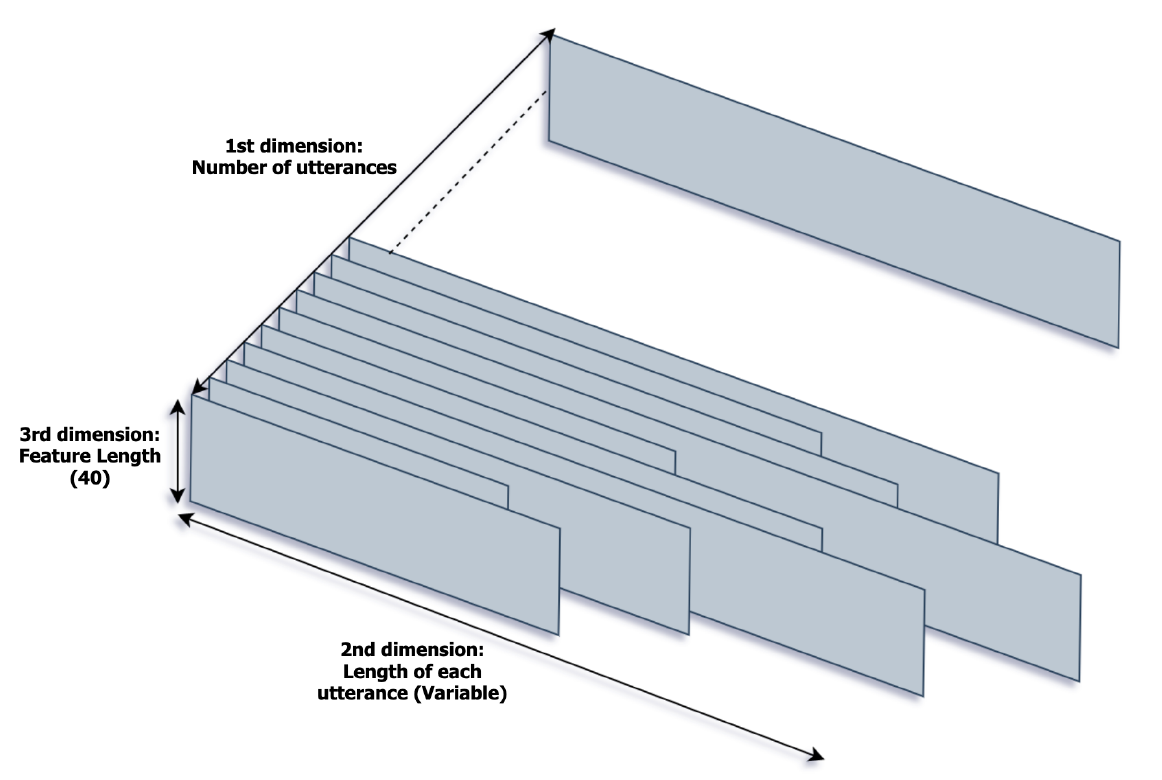
\includegraphics[width=0.5\textwidth]{images/dataset.png}
    \caption{Dataset containing mel-spectrograms.}
\end{figure}

Above is an illustration of the dataset. \\

Notice:
\begin{itemize}
    \item Each horizontal rectangle is a single audio clip (converted into mel-spectrograms).
    \item Every audio clip has a \ttt{num\_freqs} dimension of size 40 (the `height' of the rectangle)
    \item Most importantly, notice that the length (\ttt{num\_frames}) of each audio clip differs. Some utterances are long, and some are short.
\end{itemize}

In summary, each audio clip will be of shape \ttt{(num\_frames, num\_freqs=40)}, with variable \ttt{num\_frames}. \\

But we're not trying to classify audio clips - we're trying to classify each frame in each audio clip. So a batch of observations given to the NN will be shaped \ttt{(batch\_size, num\_freqs=40)}.

So there'll be one label (an integer index of the correct phoneme) for every frame of every recording in our dataset. So if there were 5 recordings in our dataset, and each contained 20 frames, there'd be 100 frames and 100 labels. \\

So predicting the phoneme for each frame seems straightforward, right? Just feed in a single frame and get a prediction for that frame. Unfortunately it's not that simple... (see next page)

\newpage
% ---------------------------------

\subsection{Adding Context}

Each frame represents just 25ms of speech. That's very short; phonemes generally take around 50-400ms, with some even taking up to 800ms. \\

So inputting and classifying just a single frame won't work. \textbf{But what if we provide some adjacent frames as context}? \\

\begin{figure}[h]
    \centering
    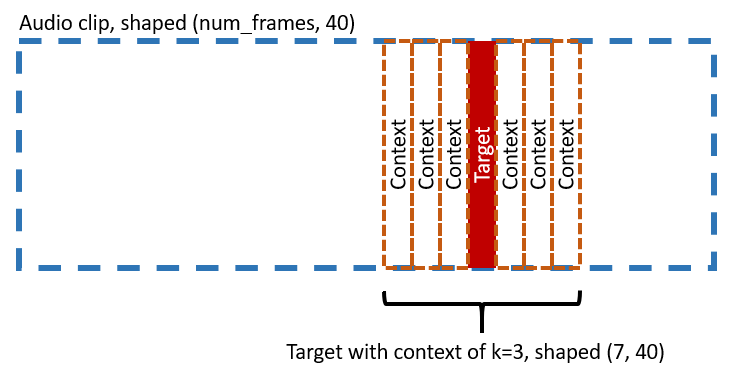
\includegraphics[width=0.6\textwidth]{images/context.png}
    \caption{Adding context}
\end{figure}

To add context, we grab \ttt{k} frames from each side and attach them to our target frame. The shape of our target along with the attached context will be \ttt{(2*k+1, 40)}, where k is the context. \\

\textbf{We'd still be predicting a single phoneme (the target frame's label)}, there's just some context around it now. \\

Also note that we've already completed this context-grabbing code for you - this description is just so you understand what's going on. \\

So with this context, how many ms do we cover now? Is it enough to capture a phoneme? \\

We can calculate how much audio we cover using this formula:

\begin{verbatim}
    num_ms(k) = stride * (2 * k + 1) + frame_width
\end{verbatim}

So if \ttt{k=3}, and given a stride of 10ms and frame width of 25ms, our observation now covers 95ms, which is a bit short. \\

See the next page for a plot of this function. \\

\newpage

\begin{figure}[h]
    \centering
    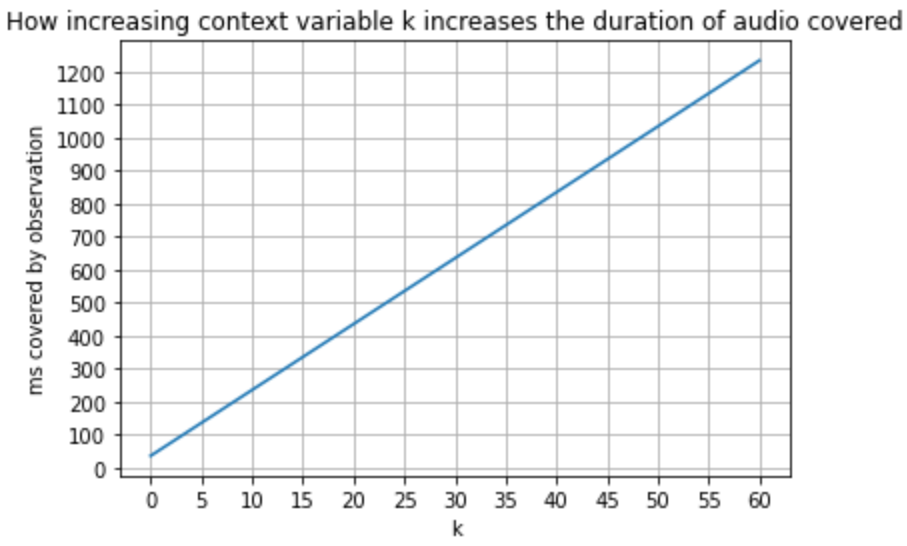
\includegraphics[width=0.6\textwidth]{images/coverage.png}
    \caption{Increasing context helps!}
\end{figure}

Start by covering around 700-800ms and increase if you need a performance boost. \\

Increasing context further will likely be beneficial but may (eventually) hurt your training:
\begin{itemize}
    \item Benefits of increasing context
    \begin{enumerate}
        \item Increasing certainty your input covers the entire target phoneme
        \item Even if you overshoot and end up including some neighboring phonemes, those neighbors may be correlated with the target phoneme (e.g. certain vowel sounds tend to be adjacent to certain consonant sounds) 
    \end{enumerate}
    \item (Eventual) Detriments
    \begin{enumerate}
        \item Slower training, due to larger inputs, larger network needed to process them, and more parameters that need to be tuned.
        \item If your input captures too many phonemes, the network will have to learn which to pay attention to and which to ignore. Likely the further away a phoneme is to your target, the less correlated it will be, meaning decreasing returns.
    \end{enumerate}
\end{itemize}

You can always start training and see how long \ttt{tqdm} (the progress bar we have set up for you) estimates an epoch will take. If it's too long, you can decrease \ttt{k} to speed things up.

\newpage
% ---------------------------------

\section{Assignment}

We've provided you a training dataset, validation dataset, and testing dataset in the \ttt{data/} folder. Notice that the test dataset is the only one without corresponding labels. \\

Your goal is to design and train a model that gets the best accuracy on a test dataset that we've hidden the labels to. \\

Here's an overview of the assignment:
\begin{enumerate}
    \item Select an architecture, optimizer, and hyperparams for your model
    \item Train for some number of epochs, validate once per epoch
    \item After an initial number of epochs trained, decide if you want to continue training
    \begin{itemize}
        \item Based on if there's still clear potential for improvement or if you're adequately satisfied with your validation performance
    \end{itemize}
    \item Given your test dataset, generating a list of predictions (one int per frame)
    \item Exporting this list to a \ttt{.csv} file and submitting it for grading.
\end{enumerate}

You may make as many test submissions as you'd like. Your grade will be determined by the highest score you achieve, even if you submit a lower score later. \\

In order to encourage friendly competition, a small part of your grade will be partially determined by the performance of your peers. You can see how they're doing on a public leaderboard. But rest assured - implementing the baseline described in the appendix and perhaps iterating on it once or twice will be enough to do well. \\

\noindent\fbox{%
    \parbox{\textwidth}{%
        \textbf{Last caveat: for this assignment, you are only allowed to use a feed-forward network that you implement yourself.} \\
        
        This means:
        \begin{itemize}
            \item No convolutional, pooling, recurrent, transformer, or geometric layers
            \item No attention mechanisms.
            \item No using pretrained DL models/ML algorithms
            \item You're encouraged to use these layers: \ttt{nn.Linear}, \ttt{nn.BatchNorm1d}, \ttt{nn.Dropout}, and any activation function you wish (except for the attention one). It's possible other layer types are acceptable, but unlikely. Focus on what we've covered in this write-up and so far in the course.
            \item The rest is fair game (e.g. batch size, optimizers, dropout percentage, weight init, class weighting in loss function, data augmentation, etc)
        \end{itemize}
    We limit your options to have you genuinely learn the fundamentals of DL. There's an ocean of obscure architectures/components, and diving in immediately generally leads to only surface-level understandings and a rip tide of bugs (ocean metaphor ends here).
    }%
}
\vspace{4mm}

\textbf{Now you can begin coding. Open the provided Jupyter notebook and follow the instructions.} \\

\newpage
% ---------------------------------

\begin{appendices}

Appendices A-D have very good info (distilled over lots of experience and research), but if you're short on time, skip to appendix E for our recommended pipeline.

\section{Layer Widths and Model Depth}

\textbf{Some rules of thumb}:
\begin{itemize}
    \item To start, make your network as wide/deep as possible given your memory/time constraints.
    \begin{itemize}
        \item To check for this, train for one iter on GPU. After backprop, your memory consumption will be largest: your weights, gradients, and data are stored on GPU. If it doesn't crash, it fits. You can also verify this by running \ttt{!nvidia-smi} and seeing how much memory is used.
        \begin{itemize}
            \item Then try running for one epoch. \ttt{tqdm} (the progress bar) will estimate how long it will take; if it's too long, you can stop the execution and reduce model size or increase batch size, and see if that helps.
        \end{itemize}
        \item Ideally, you'll overfit. This is surprisingly a good thing; it means your network has enough capacity to memorize data, which in modern DL theory, suggests potential for good learning. You can add more regularization or decrease the size of your network in response.
        \item If you underfit, consider changing architecture.
        \item If your performance is near randomness, check for bugs.
    \end{itemize}
    \item Which to increase, depth or width? Depth, but with some caveats.
    \begin{itemize}
        \item Deeper networks can be more expressive with fewer parameters.
        \begin{itemize}
            \item As discussed in lecture, a 2-layer neural network (linear, activation, linear) is a universal approximator, although it may need to be exponentially wider than the number of input features. In many modern DL problems, this is infeasible.
            \item To avoid this, we introduce depth, which significantly reduces the number of parameters needed to approximate the same function.
        \end{itemize}
        \item Caveat 1: Eventually, deep-enough networks can lead to unstable learning due to "vanishing/exploding gradients".
        \begin{itemize}
            \item This is unlikely to matter that much for this assignment, but it will in the next.
            \item There are ways to get around this problem, which you'll use eventually (but not now).
        \end{itemize}
        \item Caveat 2: If you sacrifice too much width in order to get depth, you can lose important richness of information at each layer in the model.
        \item \textbf{Solution}: Make sure each layer is just ``wide enough" and prioritize depth.
        \begin{itemize}
            \item The definition of ``wide enough" varies; see next bullet point.
        \end{itemize}
    \end{itemize}
    \item Generally, it's good to have bigger layers earlier in the network, then gradually decrease layer size as you go on.
    \begin{itemize}
        \item Your first layer could have \ttt{out\_features} $\geq \frac{1}{2} * $\ttt{in\_features}.
        \item Your second-to-last layer (layer before the output layer) should have \ttt{out\_features} $\geq$ the output layer's \ttt{out\_features}.
        \item If you restrict layer size too early or go smaller than the number of input dimensions, you force the information through a bottleneck, which may cause useful info to be lost.
        \begin{itemize}
            \item Bottlenecks aren't always bad (your own brain does this in the visual cortex), but doing it carelessly or too early in the network will likely hurt. 
        \end{itemize}
    \end{itemize}
 \end{itemize}
 
\section{Batch Normalization}
 
Batch Normalization (“BatchNorm”) is a successful and popular technique for improving the speed and quality of learning in NNs. Although its exact reason for helping is still heavily debated, it's suspected that it makes the values at each layer stabler, making the learning problem easier. \\

\subsection{How it works}

To do this, it essentially  normalizes/\href{https://en.wikipedia.org/wiki/Whitening_transformation}{\underline{whitens \ExternalLink}} the values \textit{between} layers. Specifically, a BN layer aims to linearly transform the output of the previous layer s.t. across the entire dataset, each neuron's output has \ttt{mean=0} and \ttt{variance=1} AND is linearly decorrelated with the other neurons' outputs.  \\

By `linearly decorrelated', we mean that for a layer $l$ with $m$ units, individual unit activities $ \textbf{x} = \{\textbf{x}^{(k)}, \ldots, \textbf{x}^{(d)}\}$ are independent of each other -- $\{\textbf{x}^{(1)} \perp \ldots \textbf{x}^{(k)} \ldots \perp \textbf{x}^{(d)}\}$. Note that we consider the unit activities to be random variables.\\

\textbf{In short, we want to make sure that normalization/whitening for a single neuron's output is happening consistently across the entire dataset}. In truth, this is not computationally feasible (you'd have to feed in the entire dataset at once), nor is it always fully differentiable. So instead, we maintain ``running estimates" of the dataset's mean/variance and update them as we see more observations.  \\

How do we do this? Remember that we're training on batches\footnote{Technically, \textit{mini-batches}. ``Batch" actually refers to the entire dataset. But colloquially and even in many papers, ``batch" means ``mini-batch".} - small groups of observations usually sized 16, 32, 64, etc. \textbf{Since each batch contains a random subsample of the dataset, we assume that each batch is somewhat representative of the entire dataset}. Based on this assumption, we can use their means and variances to update our running estimates. \\

\subsection{Usage Notes}

\begin{itemize}
    \item Should I put BatchNorm before or after the activation function?
    \begin{itemize}
        \item Before. Why? Google it! The community has settled on using it after the activation function, but there are strong arguments both ways.
    \end{itemize}
    \item In general Dropout and BatchNorm don't work well together.
    \begin{itemize}
        \item Why? See the abstract of  \underline{\href{https://arxiv.org/abs/1801.05134}{this paper \ExternalLink}}; TLDR, Dropout messes up the variance that BatchNorm expects.
        \item Depending on the problem space and even the researcher, they'll choose either Dropout or BatchNorm to use.
    \end{itemize}
    \item BatchNorm works differently in training mode and evaluation mode. Depending on your current task, you must toggle these modes by running `model.train()` or `model.eval()`, which will recursively set each layer to training or evaluation mode.
\end{itemize}

\section{Activation Functions}

Here's a \underline{\href{https://pytorch.org/docs/stable/nn.html#non-linear-activations-weighted-sum-nonlinearity}{list \ExternalLink}} of the various activations \ttt{torch} has available. \\

How do they differ? See this \underline{\href{https://atcold.github.io/pytorch-Deep-Learning/en/week11/11-1/}{great guide}}\footnote{And keep it a secret that we linked another course's notes here. They're just great notes!}. While you can experiment, keep it safe at first - some activations, if misused, will completely break your network, and others (probably most) will make hardly noticeable contributions. You can get top performance on this assignment with only ReLU activations.

% -----------------------------------------------

\section{Optimizers}

\subsection{Choosing an Optimizer}

Here's a \underline{\href{https://pytorch.org/docs/stable/optim.html}{list \ExternalLink}} of the various optimization algorithms you can use for stepping. \\

How do you choose and how do they differ? It gets complicated. Some of these will be discussed in lecture at some point. \\

But some general guidelines:
\begin{itemize}
    \item For most single-GPU models, there are pretty much three optimizers that are commonly used: \ttt{SGD}, \ttt{Adam}, and \ttt{AdamW}.   
    \item \ttt{SGD} is ``old but gold"; it still works remarkably well. Convergence is a bit slower and more unstable than \ttt{Adam}, but this may actually be a good thing. A common opinion in DL research today is that \ttt{SGD} has better test performance than \ttt{Adam} because it finds more robust minima.
    \item \ttt{Adam} is an overwhelmingly popular choice of optimizer in modern DL research. It converges quickly to a good solution and is relatively stable.
    \item \ttt{AdamW} is a modification on \ttt{Adam} that attempts to `fix' the way it handles \textbf{weight decay}, or L2 regularization. In practice, it seems to work very similarly to Adam, with maybe a slight improvement if you're using weight decay.
\end{itemize}

\subsection{Choosing Hyperparams (e.g. LR, Momentum, Weight Decay, etc)}

What are these hyperparameters, and how do you select them? \\

First, what are these? We'll cover these in lecture, but if anything's unclear, Google! \\

Second, how do you select them? The honest answer is `What do other people use on this dataset' and trial-and-error. But some tips:

\begin{itemize}
    \item If there's no precedent (i.e. you made this dataset or this is a private dataset for a company), you'll probably want to start from scratch
    \item If you start from scratch, you'll need to do some manual experimentation, usually with some kind of grid-search (i.e. try out various hyperparam combos, record which worked best). Alternatively, you could automatically find an LR using a package.
    \begin{itemize}
        \item For automatic LR tuning, maybe Google something like `pytorch lr finder'. There are several implementations, and they work on similar principles.
    \end{itemize}
\end{itemize}

\subsection{Schedulers}

This is another can of worms. We won't talk about them in detail, but you can find a list of them \underline{\href{https://pytorch.org/docs/stable/optim.html}{here \ExternalLink}}.


% ---------------------------------------------
\newpage

\section{Architecture Recommendations}

Now for our recommendations. If you follow this, it should be enough to do well. \\

But if you want to improve your score further, read the above appendices, identify some trends, and try making changes in the directions they suggest.

\subsection{Architecture}
Assume \ttt{LBR(X, Y)} means \ttt{Linear(X, Y) -> BatchNorm1d(Y) -> ReLU}. \\

Try 5-10 \ttt{LBR} blocks, followed by an output \ttt{Linear} layer (no activation or BatchNorm afterwards). Here's an example of what you could try:
\begin{verbatim}
   LBR(flattened_input_size, 1024) -> LBR(1024, 1024) -> LBR(1024, 1024) ->
      LBR (1024, 512) -> LBR (512, 256) -> LBR(256, 256) -> Linear(256, num_phonemes) 
\end{verbatim}

Remember, as memory allows, start by going as wide/deep as possible.

\subsection{Everything Else}
\begin{itemize}
    \item \ttt{Adam}, with default learning rate of $10^{-3}$ should suffice. You should not need to go more than an order of magnitude above or below this ($10^{-2}$, $10^{-4}$).
    \item Batch size of 1024, if it fits in memory. Anything above 256 and below 2048 should work. For now, assume the bigger the better.
    \item For most problems, the first two epochs are always the shakiest. But you can often start seeing good learning by the third epoch. 
    \item You will not need more than 10 for most of your models. If you are using above 20, you may be wasting your time.
    \item If you do decide to use dropout instead of \ttt{BatchNorm1d}, use a probability between 0.1 and 0.4.
\end{itemize}

Optionally, you can explore learning rate schedulers, which helped in our experience! \ttt{StepLR} and \ttt{ReduceOnPlateau} are great options. One way of doing things is to decay by 0.95 each epoch, another is to decay 0.1 after little change has occurred. Feel free to experiment with other schedulers!
\end{appendices}
\end{document}

